\chapter{Mission Overview and Concept of Operations}
\label{ch:mission_overview_conops}

\section{Mission Background and Motivation}
\label{sec:mission_background_motivation}

The LINKU mission addresses the study of tether dynamics in space and the development of deployment techniques for tethered satellite systems. Space tethers are relevant for applications such as passive stabilization, deorbiting, multi-spacecraft configurations, and future conductive or electrodynamic tether concepts. However, reliable tether deployment from small satellites remains technically challenging because the system behavior depends on the deployment mechanism, tether storage, relative motion, tension build-up, and the transition between slack and taut conditions.

The project focuses on a non-conductive tether as a first experimental step toward small-satellite tether technologies. This configuration allows the mission to concentrate on mechanical deployment, tethered-system motion, and passive gravity-gradient behavior. Understanding these effects provides a technical basis for future tethered-spacecraft missions, including more complex tether concepts.

LINKU combines tether-dynamics modelling, ground-based testing, and in-orbit measurements from cameras, GNSS receivers, tether-tension sensors, and spacecraft telemetry. The resulting dataset will support comparison between predicted and observed behavior during tether deployment and subsequent tethered-system motion.

The project also contributes to the development of space tether capabilities within the APSCO community by providing a collaborative framework for the study, design, and implementation of a small-satellite tether experiment.

\section{Mission Objectives}
\label{sec:mission_objectives}

The main purpose of the LINKU mission is to research tether dynamics in space and to explore deployment techniques for tethered satellite systems. These objectives support future applications of gravity-gradient satellites and contribute to the advancement of small-satellite tether technologies.

The technical objectives of the LINKU mission are:
\begin{itemize}
    \item to validate a safe tether-deployment platform for nanosatellites, based on a compact satellite architecture and a controlled SAT-B/SAT-C separation and tether-release process;

    \item to study the behavior of a non-conductive tether in orbit and to compare the in-orbit response with ground experiments and pre-flight tether-dynamics simulations;

    \item to evaluate passive stabilization behavior based on gravity gradient for its application to low-cost small-satellite systems.
\end{itemize}

These objectives are implemented through a three-spacecraft architecture in which SAT-A deploys the coupled SAT-B/SAT-C assembly, and SAT-B and SAT-C form the tethered pair used for the experiment. The measurement approach combines camera observations, GNSS-derived relative motion, tether-tension measurements, and telemetry to compare the observed behavior with pre-flight simulations and ground-test results.

\section{Mission Scenario}
\label{sec:mission_scenario}

The LINKU system is composed of three spacecraft: SAT-A, SAT-B, and SAT-C. SAT-A acts as the carrier spacecraft and accommodates the tether-experiment payload before deployment. SAT-B and SAT-C form the tether-experiment pair and become the two end bodies of the tethered system after separation.

The mission uses a consistent set of configuration names. The integrated configuration composed of SAT-A, SAT-B, and SAT-C is referred to as SAT-ABC. In this configuration, SAT-B and SAT-C are mechanically coupled and accommodated inside SAT-A. The coupled SAT-B/SAT-C assembly is referred to as SAT-BC. After SAT-BC is released from SAT-A and the SAT-B/SAT-C separation command is executed, SAT-B and SAT-C become two distinct spacecraft connected by the non-conductive tether. SAT-A then continues as an independent post-release spacecraft.

The mission scenario begins with the release of SAT-ABC from the launch deployer. SAT-ABC is stabilized and oriented for SAT-BC release. After SAT-BC deployment from SAT-A, the coupled SAT-B/SAT-C assembly is stabilized and oriented before the internal separation command. Once SAT-B and SAT-C separate, the tether is released from its storage system and the mission transitions to the observation of the deployed tethered system.

This section defines the mission at a conceptual level. The physical configuration of the spacecraft, including dimensions, accommodation constraints, and deployment clearances, is described in Chapter~\ref{ch:system_configuration}. Subsystem-level implementations are described in the payload and spacecraft subsystem chapters.

\section{Mission Concept of Operations}
\label{sec:mission_conops}

The Mission Concept of Operations describes the operational stages required to execute the LINKU tether experiment. The stages follow the configuration sequence introduced in Section~\ref{sec:mission_scenario}: SAT-ABC, SAT-BC, the SAT-B/SAT-C tethered system, and SAT-A after SAT-BC release. Each stage is divided into operational steps to identify the main activities before, during, and after tether deployment.

\subsection{Mission Stage 1: SAT-ABC Integrated Configuration}
\label{sub:conops_stage1_satabc}
In Mission Stage~1, SAT-A, SAT-B, and SAT-C are mechanically integrated and operate as the SAT-ABC configuration. After release from the launch deployer, SAT-ABC may have a non-zero initial angular rate. The objective of this stage is to reduce the tumbling motion, allow the attitude-determination solution to converge, and orient the integrated spacecraft for SAT-BC release. Figure~\ref{fig:linku_stage1} illustrates SAT-ABC in orbit and its internal accommodation arrangement.

The corresponding steps are:
\begin{itemize}
    \item \textbf{Step 1.1 -- SAT-ABC release and initialization:} SAT-ABC is released from the launch deployer and initializes its basic operational functions.

    \item \textbf{Step 1.2 -- SAT-ABC detumbling and stabilization:} The integrated configuration reduces its angular rate and reaches a stable attitude condition using the active ADCS.

    \item \textbf{Step 1.3 -- SAT-ABC settling interval:} The spacecraft remains in a settling mode to allow attitude-determination convergence and to verify that the integrated configuration is stable.

    \item \textbf{Step 1.4 -- SAT-ABC deployment orientation:} SAT-ABC is oriented along the required deployment direction for SAT-BC release.

    \item \textbf{Step 1.5 -- SAT-BC release from SAT-A:} SAT-A releases the coupled SAT-B/SAT-C assembly, which remains mechanically integrated as SAT-BC.
\end{itemize}

\begin{figure}[htbp]
    \centering

    \begin{subfigure}{0.49\textwidth}
        \centering
        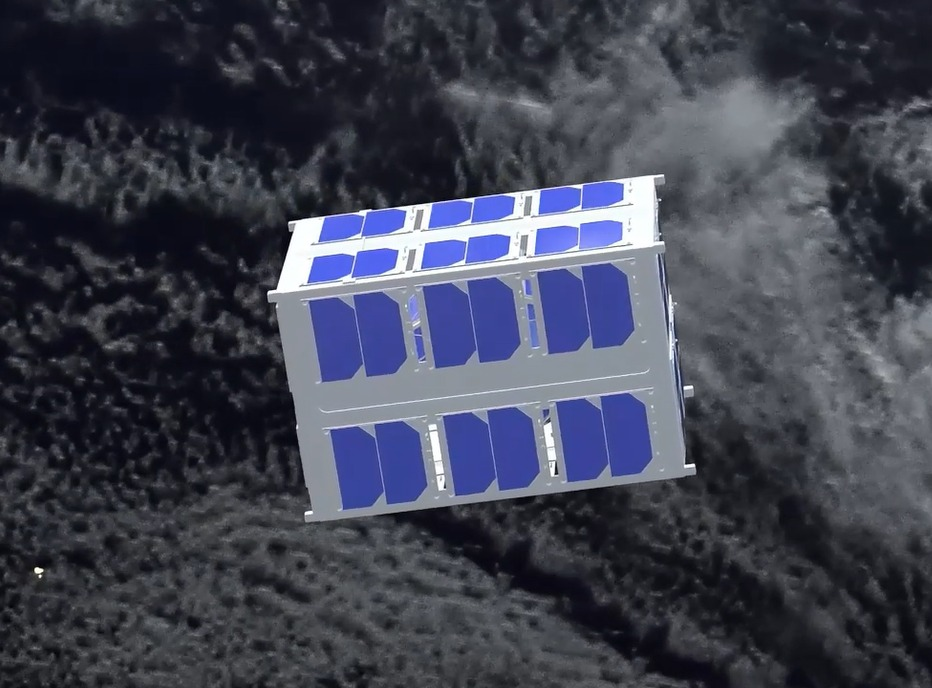
\includegraphics[
            height=5.75cm,
            keepaspectratio
        ]{SAT-ABC in Orbit.jpeg}
        \caption{SAT-ABC in Orbit}
        \label{fig:satabc_orbit}
    \end{subfigure}
    \hfill
    \begin{subfigure}{0.49\textwidth}
        \centering
        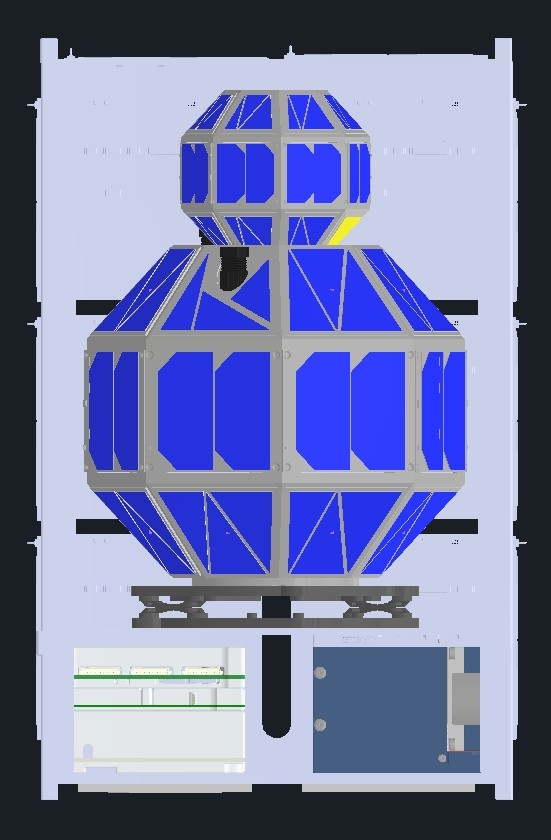
\includegraphics[
            height=5.75cm,
            keepaspectratio
        ]{Internal Layout of the SAT-ABC.jpg}
        \caption{Internal Layout of the SAT-ABC}
        \label{fig:satabc_internal}
    \end{subfigure}

    \caption{LINKU Mission Stage 1}
    \label{fig:linku_stage1}
\end{figure}

\subsection{Mission Stage 2: SAT-BC Coupled Configuration}
\label{sub:conops_stage2_satbc}
In Mission Stage~2, SAT-B and SAT-C remain mechanically coupled and operate as the SAT-BC configuration after release from SAT-A. SAT-BC may also have residual angular motion after deployment. The objective of this stage is to stabilize the coupled configuration, allow the attitude-determination solution to settle, and orient SAT-BC so that SAT-B/SAT-C separation and tether deployment occur along the intended direction. Figure~\ref{fig:SAT-BC} illustrates the SAT-BC release from SAT-A, which marks the transition from the integrated SAT-ABC configuration to the coupled SAT-BC configuration.

The corresponding steps are:
\begin{itemize}
    \item \textbf{Step 2.1 -- SAT-BC release and initialization:} SAT-BC separates from SAT-A and initializes its operational functions.

    \item \textbf{Step 2.2 -- SAT-BC detumbling and stabilization:} The coupled configuration reduces its angular rate and reaches a stable attitude condition.

    \item \textbf{Step 2.3 -- SAT-BC settling interval:} SAT-BC remains in a settling mode to allow attitude-determination convergence and stability verification.

    \item \textbf{Step 2.4 -- SAT-BC deployment orientation:} SAT-BC is oriented so that the SAT-B/SAT-C separation and tether deployment occur along the intended direction.

    \item \textbf{Step 2.5 -- SAT-B/SAT-C separation command:} The internal separation mechanism is activated to initiate SAT-B/SAT-C separation and tether release.
\end{itemize}

\begin{figure}[htbp]
    \centering
    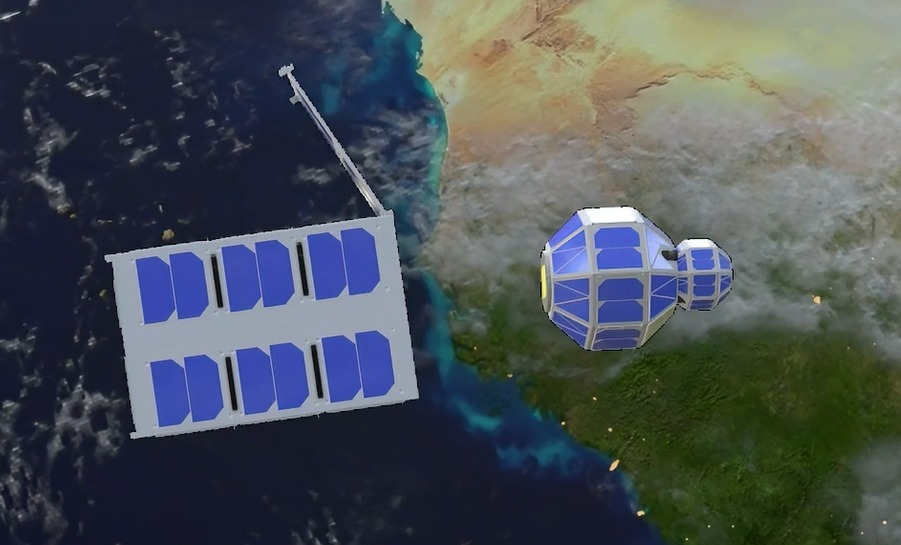
\includegraphics[width=0.65\linewidth]{SAT-BC Ejection.jpeg}
    \caption{LINKU Mission Stage 2}
    \label{fig:SAT-BC}
\end{figure}

\subsection{Mission Stage 3: SAT-B/SAT-C Tethered Configuration}
\label{sub:conops_stage3_tethered}
In Mission Stage~3, the internal separation mechanism initiates SAT-B/SAT-C separation and the tether is released from its storage system toward the nominal length of \(100~\mathrm{m}\). The objective of this stage is to observe the deployment process, the early dynamic response, and the subsequent tethered-system motion. Once the tethered configuration is established, the system transitions from the active pre-separation attitude-control stages to passive gravity-gradient-influenced behavior. Figure~\ref{fig:linku_stage3} illustrates the SAT-B/SAT-C separation process and the transition toward the deployed tethered configuration.

The corresponding steps are:
\begin{itemize}
    \item \textbf{Step 3.1 -- Tether deployment:} SAT-B and SAT-C separate while the tether is released from its storage system toward the nominal length of \(100~\mathrm{m}\).

    \item \textbf{Step 3.2 -- Dynamic transition:} The tethered system evolves through the initial post-deployment response, including tension build-up, possible slack/taut transitions, and residual oscillations.

    \item \textbf{Step 3.3 -- Tethered-system observation:} The relative motion, tether condition, and tension response are observed using the onboard measurement system to support comparison with pre-flight simulations.
\end{itemize}

\begin{figure}[htbp]
    \centering

    \begin{subfigure}{0.49\textwidth}
        \centering
        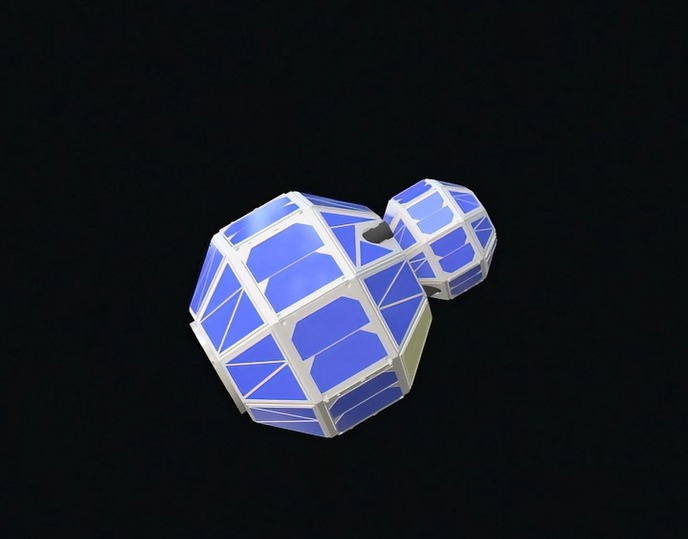
\includegraphics[
            height=5.75cm,
            keepaspectratio
        ]{SAT-B and SAT-C Together.jpeg}
        \caption{SAT-B and SAT-C together in orbit}
        \label{fig:satbc_together}
    \end{subfigure}
    \hfill
    \begin{subfigure}{0.49\textwidth}
        \centering
        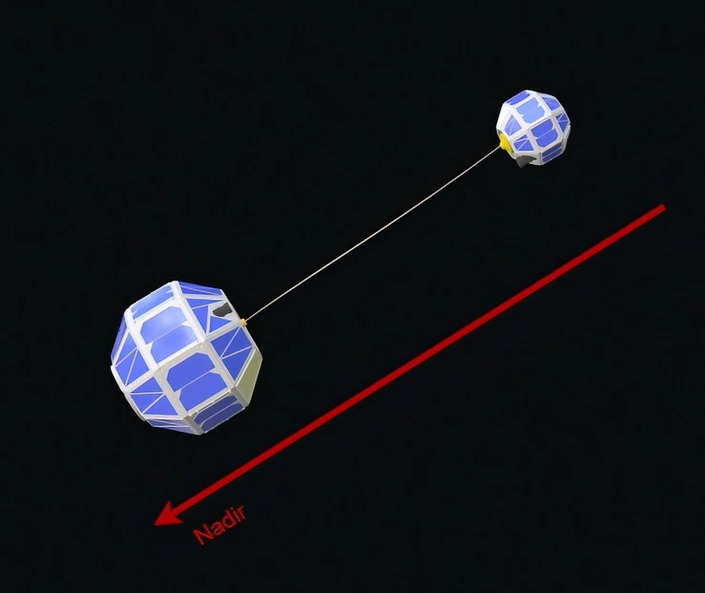
\includegraphics[
            height=5.75cm,
            keepaspectratio
        ]{Separation of SAT-B and SAT-C.jpeg}
        \caption{Separation of SAT-B and SAT-C}
        \label{fig:satbc_separation}
    \end{subfigure}

    \caption{LINKU Mission Stage 3}
    \label{fig:linku_stage3}
\end{figure}

\subsection{Mission Stage 4: SAT-A Post-Deployment Operation}
\label{sub:conops_stage4_sata_post_deployment}
In Mission Stage~4, SAT-A remains as an independent spacecraft after SAT-BC release. The departure of SAT-BC changes the mass properties and inertia of SAT-A, so re-stabilization is required before subsequent operation. The detailed definition of the SAT-A secondary mission remains outside the scope of this document, which focuses on the tether deployment and observation experiment.

The corresponding steps are:
\begin{itemize}
    \item \textbf{Step 4.1 -- SAT-A re-stabilization:} SAT-A performs a re-stabilization maneuver after the release of SAT-BC.

    \item \textbf{Step 4.2 -- SAT-A post-release operation:} SAT-A continues as an independent spacecraft. The detailed definition of its secondary mission is outside the scope of this document, which focuses on the tether deployment and observation experiment.
\end{itemize}






